\documentclass{article}
\usepackage[utf8]{inputenc}
\usepackage[margin=1in]{geometry}
\usepackage{sectsty}
\usepackage{indentfirst}
\usepackage[super]{nth}
\usepackage{graphicx}
\usepackage{subfig}
\usepackage{caption}
\usepackage{subcaption}

\usepackage[english]{babel}
%Includes "References" in the table of contents
\usepackage[nottoc]{tocbibind}


\title{An Analysis of the Applications of Computer Vision on Identifying Lost Dogs}
\author{Aidan Vickars, Anant Sunilam Awasthy, Karthik Srinatha, and Rishabh Kausha}
\date{\today}

\begin{document}

\maketitle

\newpage

\tableofcontents

\newpage
\section{Motivation and Background}
As the most common house pet, lost dogs are a frequent problem around the world.  With this is mind, it stands to reason their is no shortage of interest in new techniques for finding a lost dog.  Of course, there are a variety classical of methods that include posting flyers on telephone poles, posting adds on Craiglist and social media sites as well as leveraging purpose built applications like the BC SPCA's "Pet Search" application.  However, all of these methods require creating some form of an eye catching poster or description that has been used in so many different forms that they have lost their intended affect.  As a result, a new method is needed.  Thus, in this paper we will present a data pipeline implemented as an Android Application that leverages three separate convolutional neural networks to match lost dog and found dogs together.  We do this by computing the similarity between lost and found dogs and subsequently returning the most similar results to the user.

\section{Related Work}
	While dog-identification is a sub-class of the heavily researched facial recognition area, dog-identification remains extremely undeveloped.  However, there are two related works that we discuss here.  The first is "A Deep Learning Approach for Dog Face Verification and Recognition" \cite{MougeotGuillaume2019ADLA}  by  Guillaume Mougeit, Dewei Li and Shuai Jia.  In this paper, Mougeit, Li and Jia present "VGG-like and "ResNet-like" (page 422) models that encode the image of a dog and compute the Euclidean distance between the encodings to measure the similarity between two dogs.  This value is used to perform face verification to determine if two dogs are the same.  To quantify the accuracy of their models they generated 2500 positive pairs and 2500 negative pairs of images.  In this scenario positive indicates the images represent the same dog and negative indicates the images represent different dogs.  Their models made the correct decision 92\% and 91\% of the time for each model respectively.

	The second work is "Dog Identification using Soft Biometrics and Neural Networks" \cite{LaiKenneth2019DIuS} by Kenneth Lai, Xinyuan Tu and Svetlana Yanushkevich.  In this paper, Lai, Tu and Yanushkevich present an approach to increase the accuracy in dog-identification that is the inspiration behind the work presented here, and all credit is given with respect to the similarities between our works.  Lai, Tu and Yanushkevich developed a dog detection model, a breed classification model, and a dog-identification model that work together in the order specified.   The dog detection model determines the bounding box of the face of a dog and can be used to crop the image accordingly.  The breed classification model like other models of this type, simply determines the most likely breed of the dog.  Finally, the dog-identification model functions in the same way as the models created  Mougeit, Li and Jia discussed above.  By first cropping the image, and filtering by the breed of the dog, the number of comparisons that are made using the dog-identification model is significantly reduced and the face verification accuracy is improved.  However, we do not state the accuracy of the models as the dog-identification model is trained on the "Flickr-dog" \cite{LaiKenneth2019DIuS} data-set that contains only 374 images made up of just two breeds.  As a result, our findings are incomparable.

\section{Problem Statement}
	It should be noted that in both papers discussed above, the dog-identification models are trained and test on highly curated images that contain only the face of a dog.  To be succinct, the entire body of the dog is cropped out and the remaining face is normalized by horizontally aligning the image according to the dog's eyes.  Images that do not contain the dogs face are removed.  This presents a deficiency in two ways.  The first is that by training the model on such a highly curated data-set, the assumption is made that all applicable images contain the dog's face in a relatively front facing fashion.  This is obviously not the case.  Any dog owner knows convincing your dog to look at the camera is a non-trivial task and that the majority of their photos are of the dog in an appealing position with their face obscured.  An example of this is shown in Figure \ref{fig:x dog no face} below.  


\begin{figure}[h]
\centering
	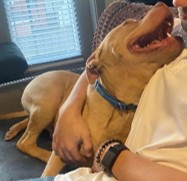
\includegraphics{final-report-images/nofacedog.jpg}
\caption{An Example of a Dog with their Face Obscured}
\label{fig:x dog no face}
\end{figure}
\newpage

The second deficiency is that by cropping the image to only the dogs face we theorize that valuable information is lost.  In the case of face verification in humans, only examining the face is desirable because humans change clothes.  However, dogs do not.  We certainly note that there are cases where dogs do wear clothes but these cases are infrequent.  Thus, we theorize that by leveraging a dogs entire body we may see an improvement in the accuracy of the dog-identification model relative to work done by  Lai, Tu and Yanushkevich.  This is because the model could leverage additional characteristics such as the size and shape of the dog.  This is illustrated in Figures \ref{fig:x similar faces} and \ref{fig:x different bodies}.  In Figure 2 the two dogs have very similar faces; one could forgive a model for classifying these dogs as the same.  But in Figure 3 we can clearly see that are not.  By leveraging the entire body of dog, this miss-classification should be eliminated.

\begin{figure}[h]
\centering
	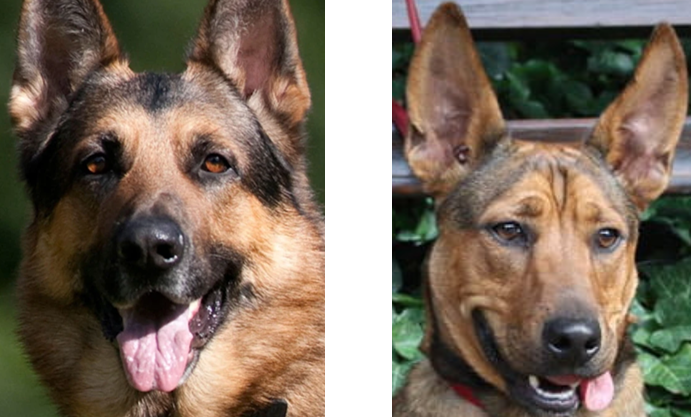
\includegraphics{final-report-images/similar_faces.png}
\caption{Two Dogs with Similar Faces}
\label{fig:x similar faces}
\end{figure}

% \newpage

\begin{figure}[h]
\centering
	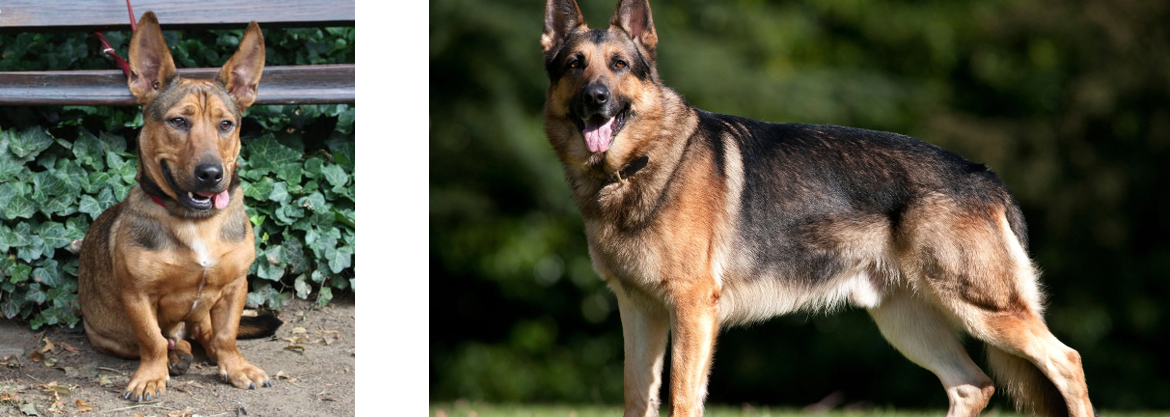
\includegraphics{final-report-images/different_bodies.png}
\caption{Two Dogs with Similar Faces but Different Bodies}
\label{fig:x different bodies}
\end{figure}

Thus, we can now present the key problems this project aims to answer:

\begin{enumerate}
  \item By leveraging the entire body of a dog, can we construct an dog-identification model that can accurately determine if two dogs are the same or not?  Furthermore, can we achieve a better accuracy than that achieved by Mougeit, Li and Jia?
  \item By removing the restriction of curated front facing dogs, can we construct a pipeline that can accurately match lost dogs and found dogs together? 
\end{enumerate}

\section{Data Product}

	To answer the questions stated above, we use the work done by Mougeit, Li and Jia and use a similar VGG model to compare dogs and we also incorporate the work done by Lai, Tu and Yanushkevich and create a dog localization model and breed classification model to improve accuracy.   We extend this by using the entire body of a dog instead of the face to remove possible miss classifications as explained above.  In future references we refer to the these models as the Dog Comparator, the Dog Extractor and the Dog Classifier respectively.  However, before elaborating on each individual model we will present the Data Product to give the reader context as to how the models work together.

	To utilize this work in a production environment, we have created an android application (app) to act as user interface to allow for easy image upload, and have packaged the models inside a Flask API to match lost and found dogs together. We also use an AWS S3 bucket and a Relational Database System to store images and image metadata respectively.  This system is visualized below in Figure \ref{fig:x app system}.

\begin{figure}[h]
\centering
	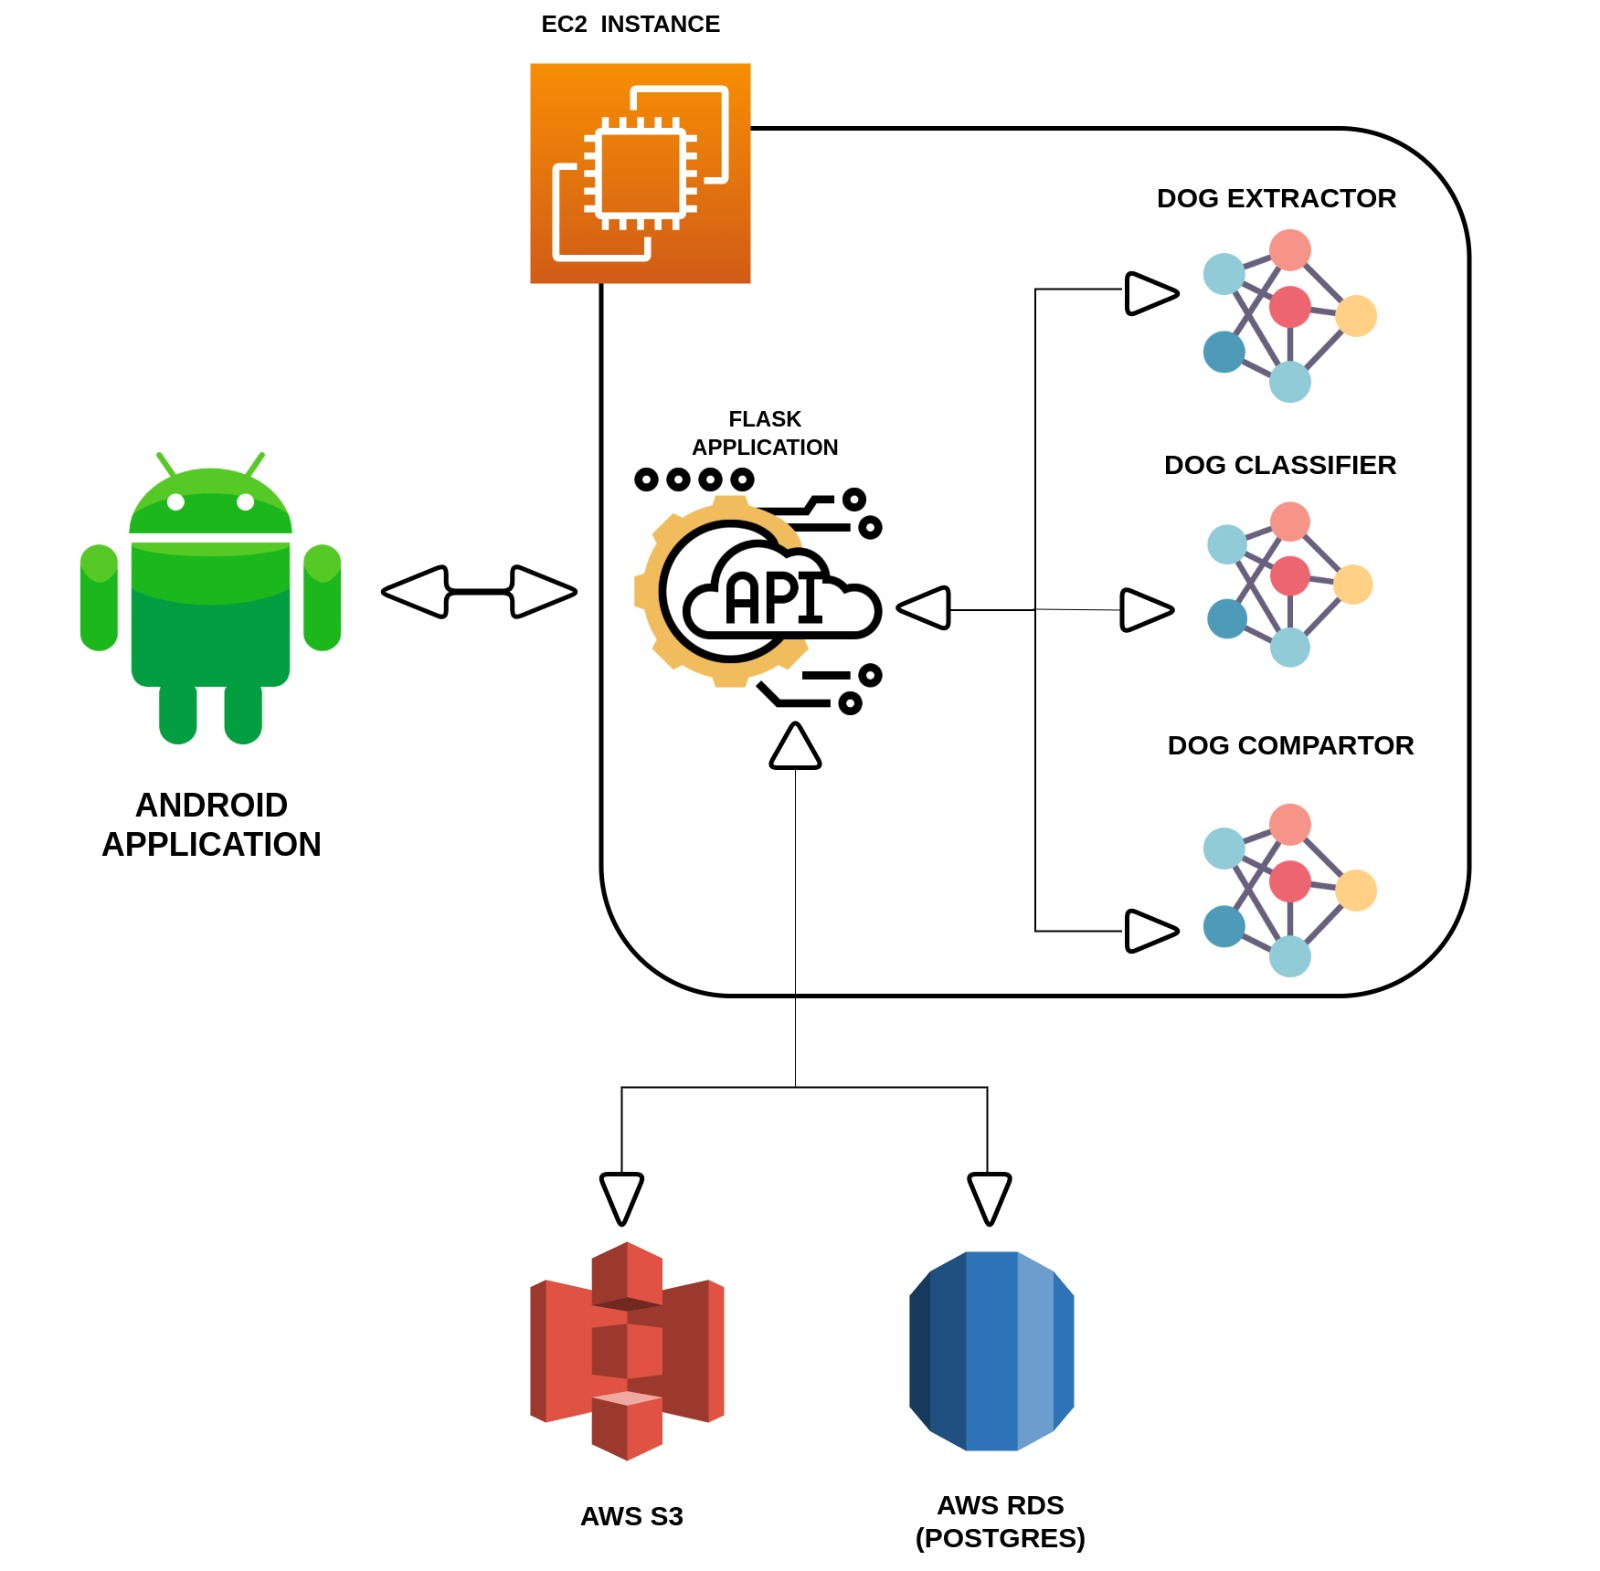
\includegraphics[scale=0.1]{final-report-images/system.jpeg}
\caption{Dog Finder System}
\label{fig:x app system}
\end{figure}

At a lower level if the user has lost a dog, they will submit a photo and their contact information and location via the app.  The app will then submit this information to the API.  Once a submission has been made to the API, the dog finder pipeline that is visualized below in Figure \ref{fig:x app pipeline} is triggered.  The following steps outline this pipeline:
\newpage

\begin{figure}[h]
\centering
	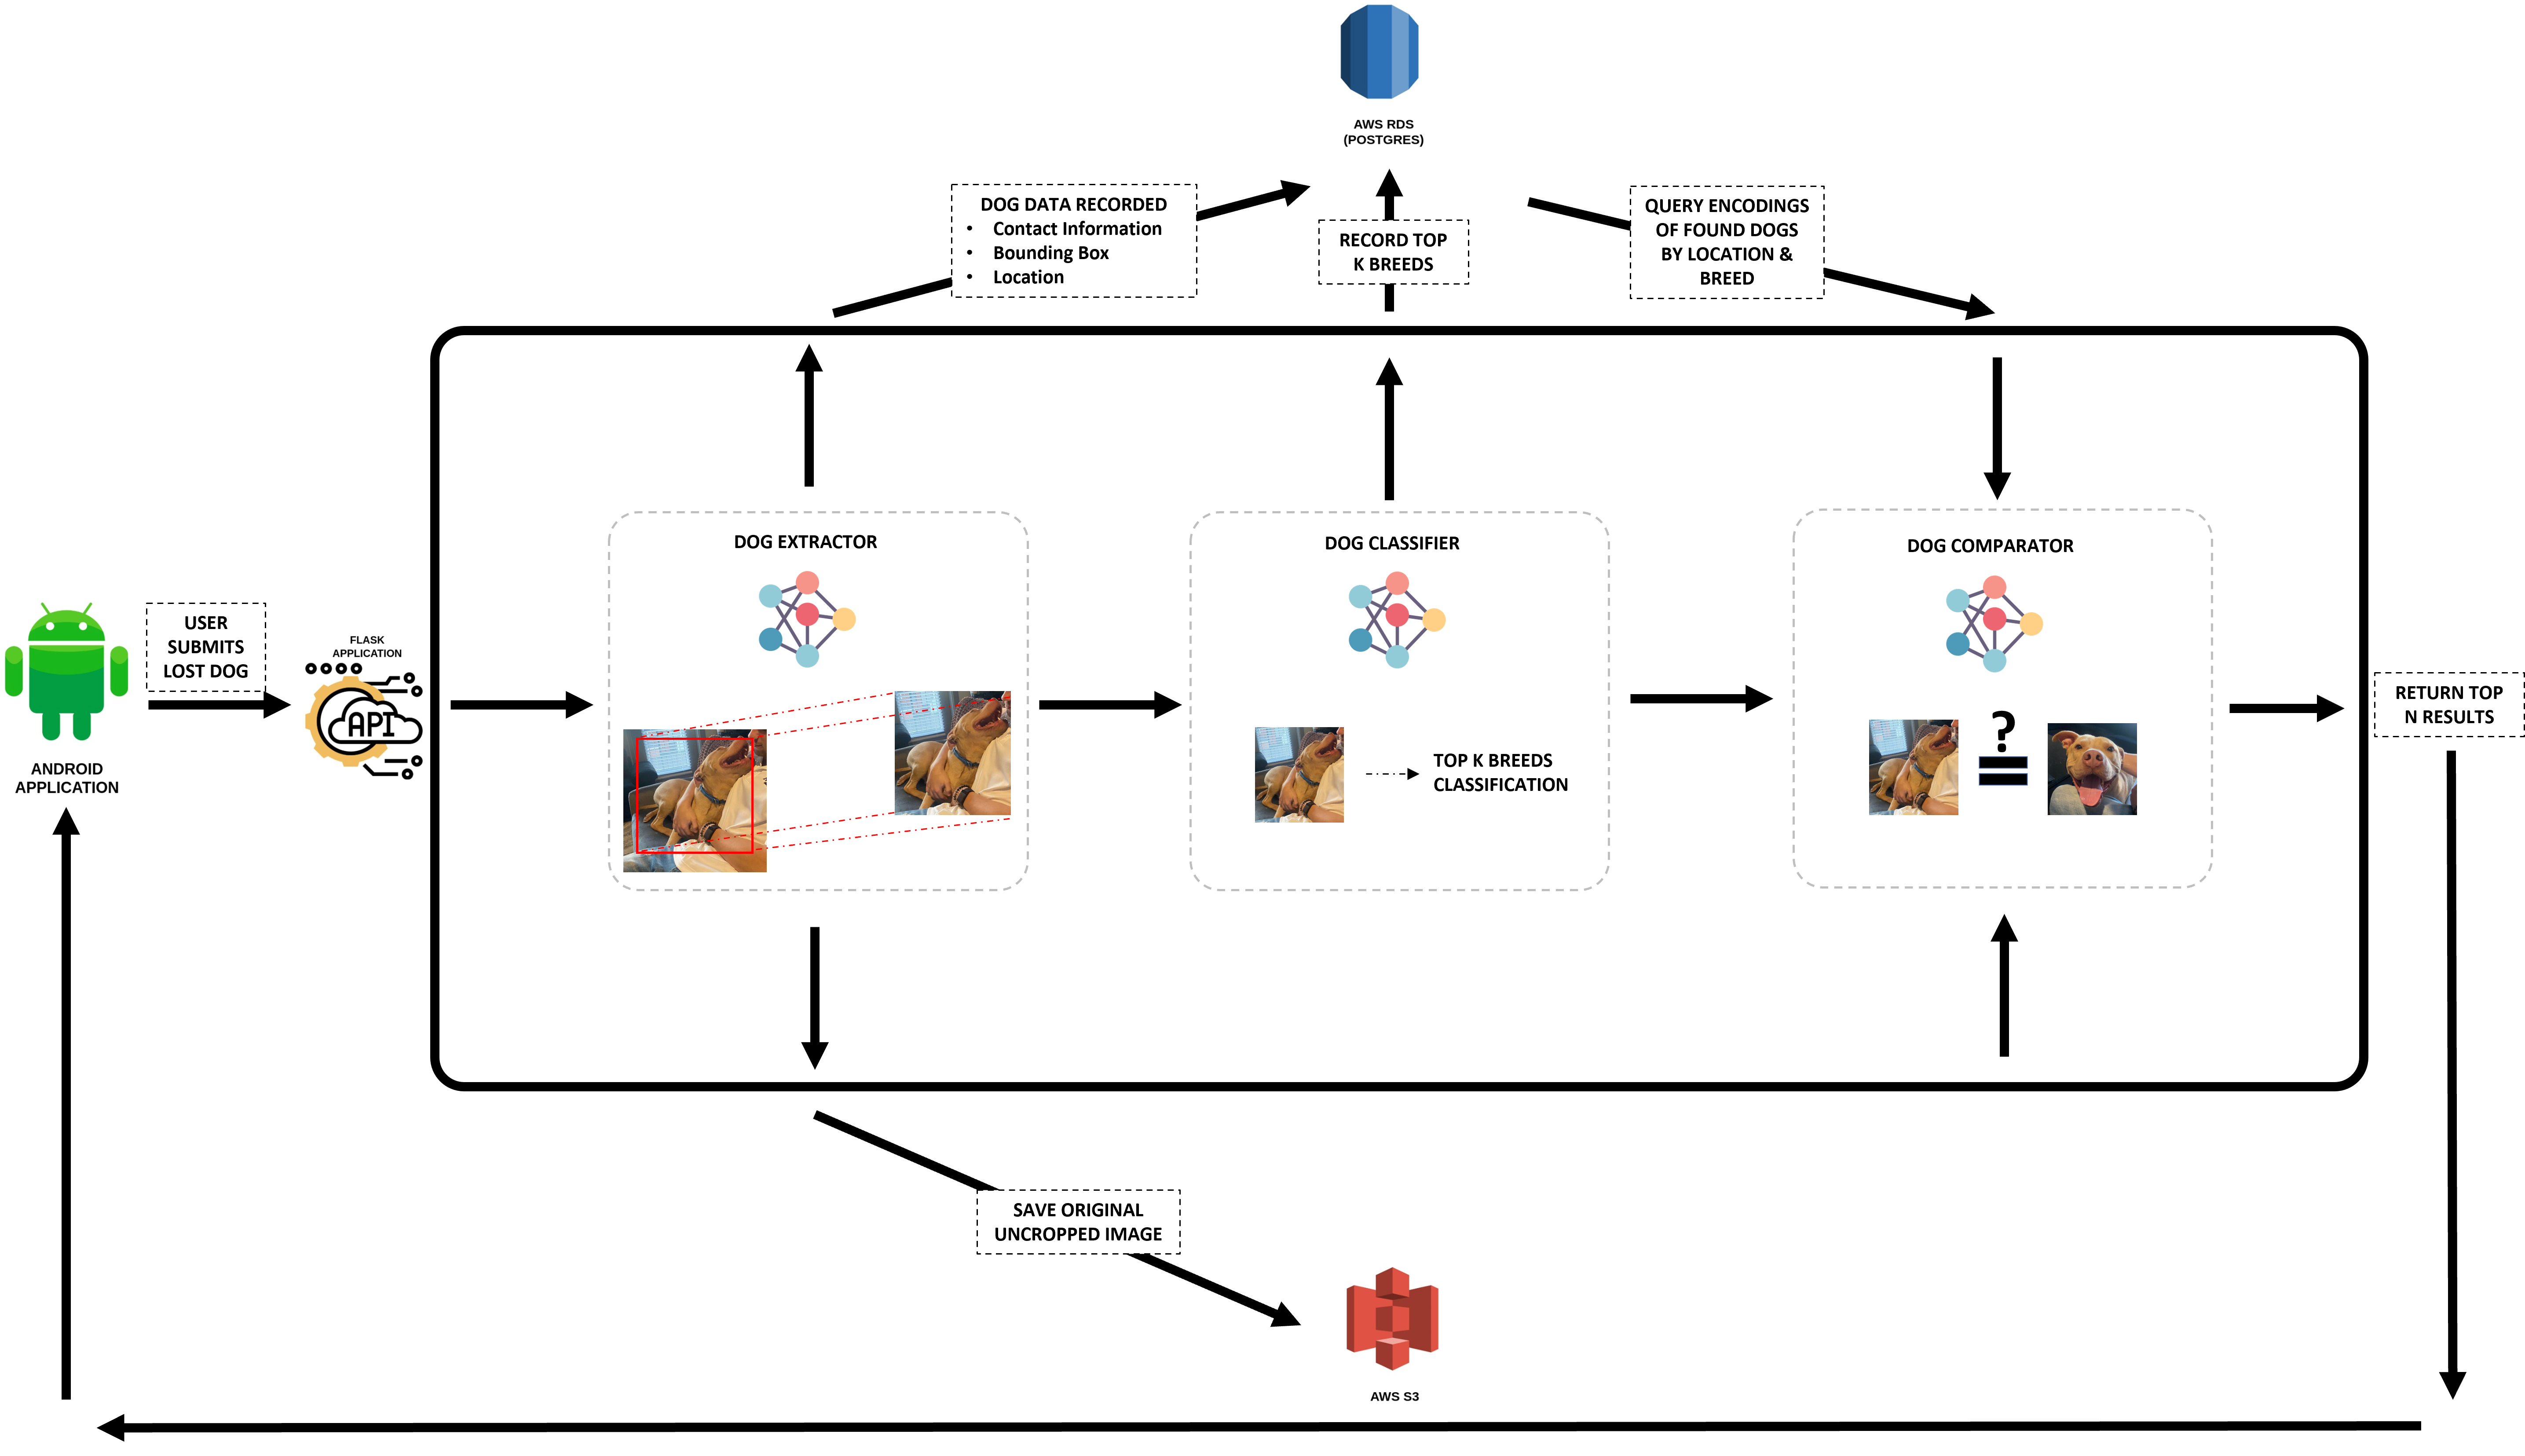
\includegraphics[width=1.0\textwidth]{final-report-images/applowlevel.png}
\caption{Dog Finder Pipeline}
\label{fig:x app pipeline}
\end{figure}

\begin{enumerate}
  
  \item Once a lost dog has been submitted, the image is passed to the Dog Extractor model that computes the coordinates of the bounding box of the dog.  This model also acts as a quality control by validating the image to ensure that the it contains a dog, and only one dog.  If these conditions are not met, an error is returned to the user.
  
  \item After validation, the original image is saved into an S3 bucket, and the related information such as the users contact information, location and the coordinates of the bounding box are inserted into a PostGre relational database system (RDS).
  
  \item The original image is then cropped using the computed bounding box coordinates, and passed into the Dog Classifier model that determines the most likely breed(s).  This information is inserted into the RDS.
  
  \item The cropped image is also passed into the Dog Comparator model that creates a five dimensional encoding of the image that is inserted into the RDS.
  
  \item We then query the encodings of the dogs marked as found according to:
  
  \begin{enumerate}
      \item Dogs that have at least one breed in the intersection between their $b$ most likely breeds respectively, and the $m$ most likely breeds of the lost dog.
      \item Dogs that are within $x$ distance from the lost dog.
  \end{enumerate}

   These encodings are then compared against the encodings of the lost dogs by computing the euclidean distance between them.  The sigmoid function is applied to the distance value to constrain it to $[0,1]$.  The $n$ most similar dogs are returned to the user.
  
  \item If a match is confirmed by the user, the corresponding lost and found dogs are removed from the RDS and S3 bucket.  Otherwise, the lost dog is left in the system for future comparisons.
 
\end{enumerate}

An attentive reader will notice that we discuss only the submission of lost dogs.  This is done to minimize confusion.  If the user submits a found dog the pipeline is identical except that the dog is instead marked as found and is compared against lost dogs.  This completes the pipeline contained within the application. 

\section{Data Science Pipeline}

\subsection{Open Images Data-set}

To train each model, we leveraged three different data sets for each model respectively.  For the Dog Extractor model, we utilized the "Open Images" \cite{openimages} data-set that contains thousands of images of dogs with corresponding bounding boxes.  While this data is already relatively clean, we discarded all grey-scale images, and converted all images to RGB format.  The decision was made to discard grey-scale images because our expectation is that in the production environment of the app, the vast majority of images will be colour images.  After cleaning this left 19 995 training images, 1568 validation images , and 4791 test images.

\subsection{Dog Classifier Models Data-set}

For the Dog Classifier Model ---------------------

\subsection{Petfinder Data-set}

Finally, to train the Dog Comparator model we required multiple pictures of many individual dogs where each picture contained the entire body of the dog.  However, we found that there was no data-set that met these requirements.  We note that the "Stanford Dog Data-set" \cite{stanforddogs} contains multiple images of 1425 individual dogs.  However, each image contained only the face of a dog and the images appeared to be highly curated.  We found the images to be front facing and highly normalized which as discussed above is undesirable.  To solve this we scraped the trove of images on Petfinder.com that at the time of writing lists over 100 000 dogs for adoption across the world where almost every dog has multiple images.  However, scraping the images presented a challenge because the links to every dog are dynamically generated.  This meant scraping the HTML of the web page containing the grid of available dogs using Python's request package was insufficient because during download the URLs pointing to each available dog would not be included due to their dynamic creation.  To solve this, we split the scraping into two parts.  We first created a Selenium application in Python that scraped the URLs pointing to each individual dog.  Then, using these URLs we scraped and downloaded the images for every dog and also recorded additional information such as name, breed, age, size etc.  This resulted in images for 9729 dogs with 0 - 6 images for every dog.  Once the data was downloaded, we applied the following cleaning process on the images of every dog:
\begin{enumerate}
  
  \item If the dog has 1 or a less images, we discarded the dog and its images.
  
  \item Confirmed every image was in RGB format or convert it to RGB format.  Otherwise the image was discarded.
  
  \item Passed every image into the Dog Extractor Model:
    \begin{itemize}
      \item Verified the image contained a dog.
      \item Verified the image contained only one dog.
      \item Recorded the bounding box coordinates of the dog.
    \end{itemize}
    If either of the conditions in the first two bullets were not met, the image was discarded.
    
  \item If after the previous step, the Dog had 1 or less images we discarded the dog and its images.
  
\end{enumerate}

\noindent After cleaning we were left with 8349 dogs with 2 - 6 images for every dog.  The data set was then divided into a Train, Validation and Test split of 70\%, 10\%, and 20\% respectively.  This gave a total of 6679 training dogs, 501 validation dogs and 1169 testing dogs respectively.  We do note that we did not account for the actual number of dog images contained in each split.  This is because during the training and testing process we only considered the images on a dog by dog bases.  This will become more clear in the presentation of the Dog Comparator model below.

After applying the above cleaning steps, we further processed the data by parsing the breed of each dog.  We found that while the breed was available for most dogs in the data-set, it could be in many forms such as "German shepherd dog" and "terrier" where capitalization was not consistent and inconsequential words like "dog" were contained in the breed.  Furthermore, the data-set contained mixed breeds that were in the form of "German shepherd \& terrier".  This meant that the breeds needed to be standardized.  We did this by applying the following steps:

\begin{enumerate}
  \item Converted all strings to lowercase.
  
  \item Removed inconsequential words like "mixed", "breed", and "dog".
  
  \item Split the breed into two strings using '\&' to account for mixed breeds.
    
  \item Compared the list of breeds against the  standardized list of 120 breeds contained in the "Stanford Dogs Data-set" \cite{stanforddogs}:
    \begin{enumerate}
      \item Computed the cross product between the two lists.
      \item Computed the Jaccard similarity between every pair.
      \item Removed any pairs with a similarity less than 0.75.
    \end{enumerate}
\end{enumerate} 

\noindent By doing this, we successfully standardized the breeds contained in the data-set.  The reader may notice that dogs without a breed were not removed.  This is because during the initial training of the Dog Comparator model as discussed below, we did not require the breed.  During testing, dogs without a breed we removed when required.

\section{Methodology}
Now that the data-sets used have been outlined, the approaches used in each model can be discussed.  For all three models, we present the architecture used and their respective results.  We also perform a deep analysis into the strength and weaknesses of each model respectively.  

\subsection{Dog Extractor}

To develop the Dog Extractor model, we investigated multiple avenues that included developing an original implementation of a transfer learning approach to Yolo V2 \cite{RedmonJoseph2016YBFS}.  However, we found a significant limiting factor to be a lack of GPU memory.  To be succinct, we trained the Dog Extractor model on an RTX 3070 with only 8 GB of memory.  Because we wanted to use larger and more complex models to achieve high degrees of accuracy, our models would train very slowly due to the requirement of having a very small batch size during training because of memory limitations.  This necessitated the requirement to utilize a largely pre-trained model via transfer learning and only make small adjustments with minimal amounts of additional training.  To achieve this we employed transfer learning using a pre-trained Faster RCNN \cite{DBLP:journals/corr/RenHG015} model using PyTorch with a feature extractor trained on the COCO data-set \cite{coco} to act as the back bone of the network.  We adjusted the output of the model from predicting a multitude of classes to only two and in doing so converted the model to a dog localization model.  In short, the model was adjusted to predict only the background class and the dog class.  In case the reader is unfamiliar with object localization models, we give a brief description of the model input and output.  The dog localization model accepts an image as input, and outputs a list of bounding box proposals and object score pairs.  Each pair gives the coordinates of a bounding box surrounding the object and the confidence that the box contains a dog respectively.  This list is subsequently passed into the Non Max Suppression algorithm \cite{nms} that filters out overlapping proposals and proposals with low degrees of confidence.  If the reader is unfamiliar with NMS, we present the algorithm here: \\

\begin{minipage}{1\textwidth}%
	\noindent \textbf{Non Max Suppression Algorithm} \\

  \noindent \textbf{Input:} List of bounding box proposals and object score pairs. \\
  
  \noindent \textbf{Output:} Filtered list of bounding box proposals and object score pairs \\
  
  \noindent \textbf{Algorithm:} \\
\end{minipage}%

\begin{enumerate}

  \item Initialize empty list, lets call it list B.

  \item Order the bounding boxes and object score pairs according to the object score in descending order.
  
  \item Discard any pairs whose object score is less than the pre-defined object threshold.  Bounding boxes with an object score lower than this threshold likely do not bound anything or do so poorly.
  
  \item While there are still bounding boxes and object score pairs on the list:
        \begin{itemize}
             \item Pop the first pair off the list and record it in list B.
            
             \item Compute the intersection over union (IOU) between the pair just popped off the list, and all remaining pairs on the list.
             \item If the resulting IOUs are greater than the predefined IOU threshold, discard the corresponding pairs.  The bounding boxes of these pairs likely bound the same dog.
        \end{itemize}
\end{enumerate}


The model was trained on the cleaned "Open Images" data-set for 10 epochs with an initial learning rate of 0.005 and a decay of 0.1 every 3 epochs, as well as a momentum value of 0.9.  Due to memory limitations, our batch size was set to one.  We note that PyTorch's tutorial on object detection \cite{TorchVision} was very helpful here and we give all credit accordingly.  During training we concerned ourselves only with the validation Mean Average Precision (MAP) because we are concerned only with a single class.  We coded and computed the MAP over an IOU threshold range from 0.5 to 0.95 in increments of 0.05, and computed the mean.  We denote this value as MAP 0.5:0.95.  During training we saved the model weights only when the MAP 0.5:0.95 increased and achieved a best validation MAP 0.5:0.95 of 0.73 during training using an object score threshold of 0.6 and an IOU threshold of 0.5 in non max suppression (NMS).  The MAP 0.5:0.95 is plotted below in Figure \ref{fig:x epoch_v_map} over 10 epochs. 

\begin{figure}[h]
\centering
	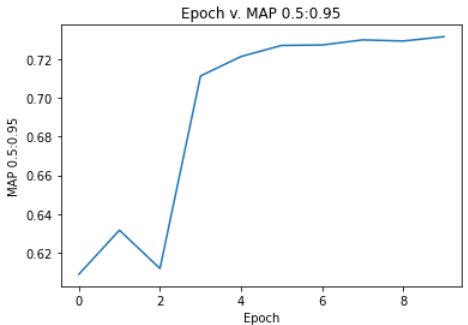
\includegraphics[scale=0.7]{final-report-images/epoch_v_map.png}
\caption{Epoch vs. MAP 0.5:0.95}
\label{fig:x epoch_v_map}
\end{figure}

To improve the accuracy of the model we tune the object score and IOU thresholds used in NMS.  To do this we used a brute force approach by applying NMS on the model output on the validation data over a grid of object score and IOU thresholds and then computed MAP 0.5:0.95 on the results.  We used a large grid that ranged from 0.05 to 0.95 for both thresholds.  The results are visualized below in Figure \ref{fig:x object v iou}.  

\begin{figure}[h]
\centering
	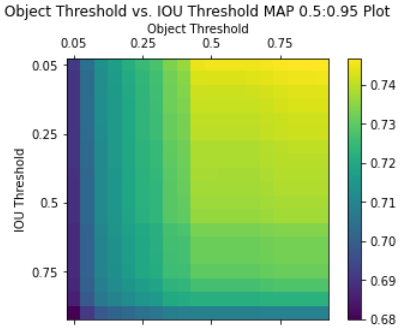
\includegraphics[scale=0.7]{final-report-images/map0.5to0.95.png}
\caption{Object vs. IOU Threshold MAP 0.5:0.95}
\label{fig:x object v iou}
\end{figure}
\newpage
\noindent We achieved the maximum MAP 0.5:0.95 of 0.75 in the top right corner of the plot using an object threshold of 0.05, and an IOU threshold of 0.9.  However, we consider the consequences of using such extreme thresholds.  By using such a low object threshold, many more bounding box proposals will be returned by NMS regardless of how uncertain the model is that there is a dog in the bounding box.  This will increase the number of false positives the model produces.  In a similar fashion, by using a strong IOU threshold of 0.9 any pair of bounding boxes must achieve an IOU greater than 0.9 to be classified as bounding the same dog.  This will again increase the false positive rate.  In the context of the app, this will significantly increase the number of errors users receive when submitting an image.  This is because every image submitted is validated to ensure it contains only one dog.  Thus, by increasing the false positive rate the number of errors returned to the user would likely increase significantly.  To combat this, we deviate from the optimum thresholds and increase the object threshold to 0.5 and decrease the IOU threshold to 0.75.  This combination achieves an MAP 0.5:0.95 of 0.74.  A very small decrease of just 0.01.  Finally, using our chosen thresholds, the model achieves an MAP 0.5:0.95 of 0.74 on the test data indicating the model performs very well.

\subsection{Dog Classifier}

\subsection{Dog Comparator}
To create the dog comparator model that assesses the similarity between two dogs, we leveraged the pre-trained feature extractor from the VGG 19 classifier \cite{SimonyanKaren2014VDCN} and added three additional layers.  This is visualized in Figure \ref{fig:x comparator} below.

\begin{figure}[h]
\centering
	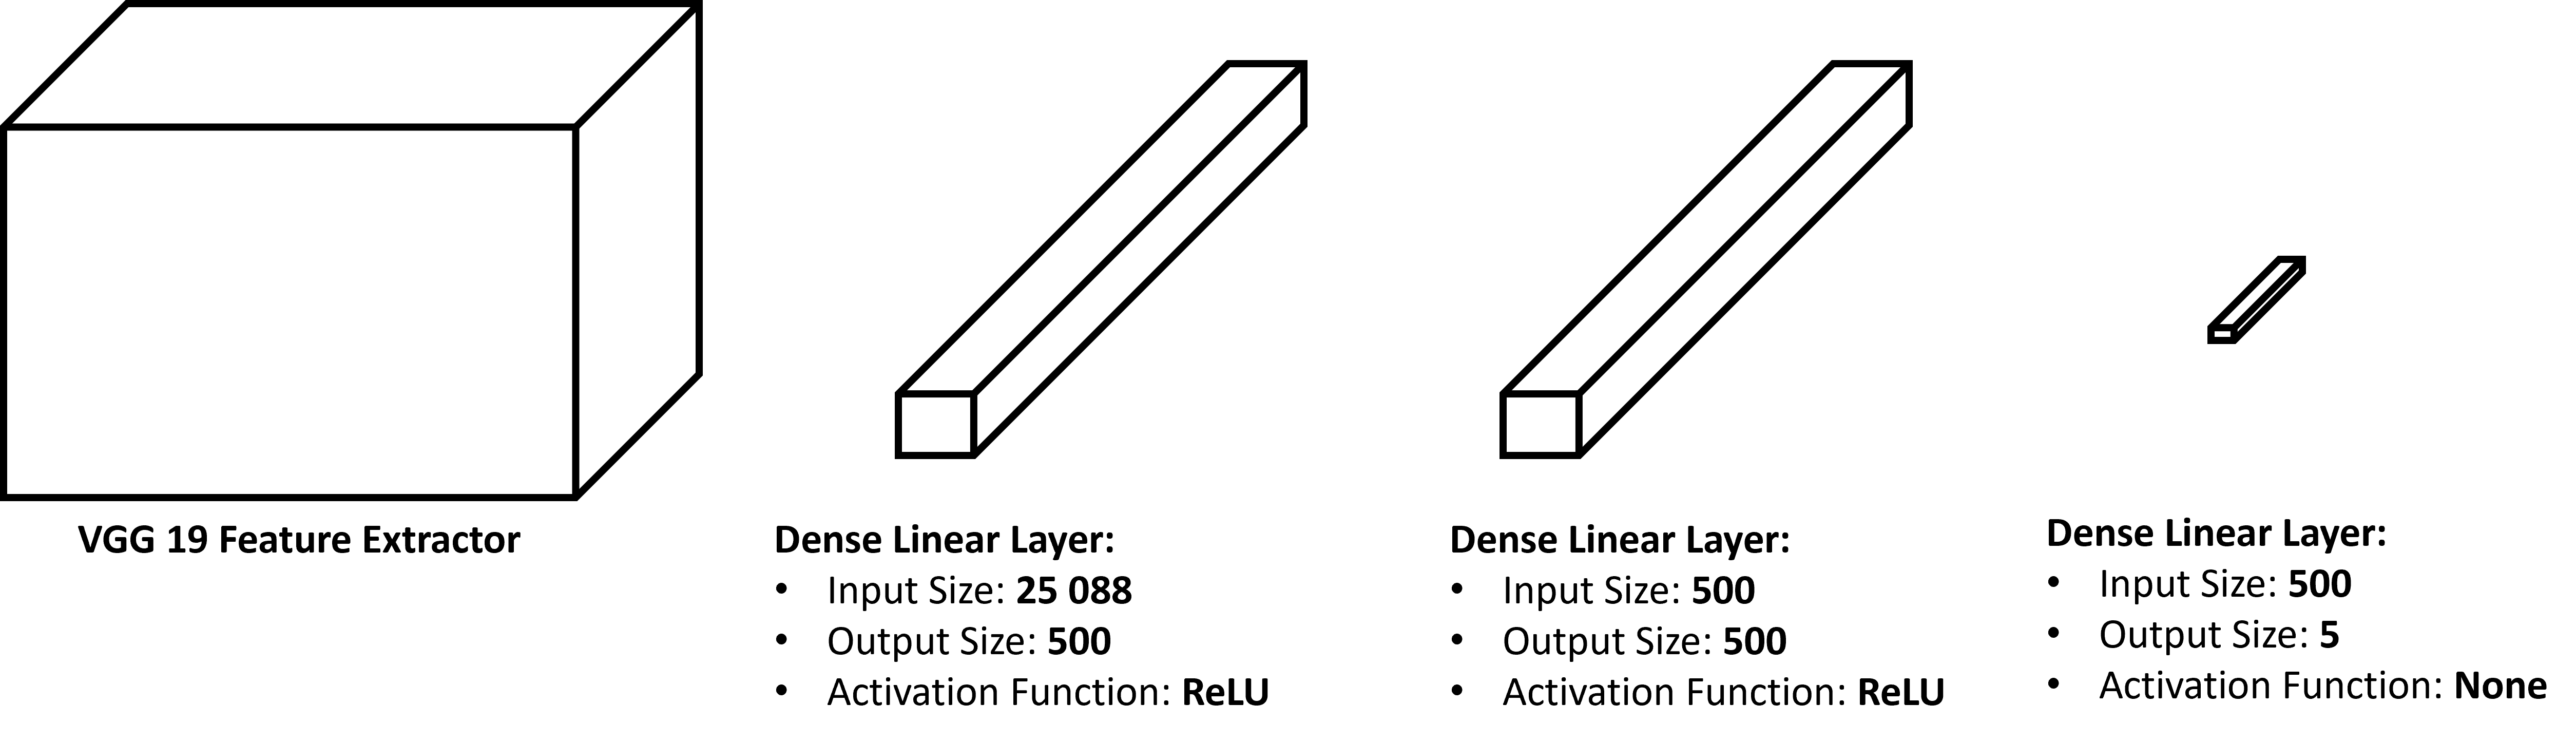
\includegraphics[scale=0.4]{final-report-images/dog_comparator.png}
\caption{Dog Comparator Model Architecture}
\label{fig:x comparator}
\end{figure}

\noindent When an image is passed through the model, a five dimensional encoding of the image is produced.  To compute the similarity between two dogs, the euclidean distance between their encodings is computed.  The sigmoid function is then applied to constrain the value to $[0,1]$ .  We can call this value the similarity value.  If two dogs are very similar, their encodings should be relatively close together in the five dimensional space.  As a result, the distance between them and the similarity value should be close to zero.  In contrast, if two dogs are very dissimilar the distance between them should be large and the resulting similarity value should be close to one.  

To train the model we employed a triplet loss function that required a batch element that contained three images.  An anchor and positive image that contained different pictures of the same dog as well as a negative image that contained a different dog.  To generate a single batch element we used the following process: \\

    \begin{minipage}{1\textwidth}%
      \noindent \textbf{Input:} Index of a dog in the data-set \\
      
      \noindent \textbf{Output:} Positive Image, Negative Image, and Anchor Image \\
      
      \noindent \textbf{Algorithm:} \\
    \end{minipage}%
    
    \begin{enumerate}
    
      \item Randomly choose two different images of the indexed dog.  Assign one image as the positive image and anchor image respectively. 
    
      \item Randomly select a different dog, and randomly select an image of the dog.  Assign this image as the negative image.
      
      \item Return the positive, anchor and negative images.
    
    \end{enumerate}

Each image was then passed through the model and the loss was computed.  In case the reader is unfamiliar with the triplet loss function,  it is defined as $L(P, A, N) = ReLU(\sigma(Dist(P, A)) - \sigma(Dist(P, N)) + M)$ where $P, A$ and $N$ are the positive, anchor and negative images respectively, $Dist()$ is the euclidean distance between their encodings, $\sigma()$ is the sigmoid function and $M$ is the margin that was set to 0.9.  Note, an attentive reader will notice the large decrease in dimension in the first dense layer.  This was done to accommodate GPU memory limitations so that the batch size could be increased during training.   The model was trained for 41 epochs with a learning rate of 0.01 that decayed by 0.1 every four epochs as well as a batch size of 30.  The training and validation losses are vizualized below in Figure \ref{fig:x epoch_v_map} .

\begin{figure}[h]
\centering
	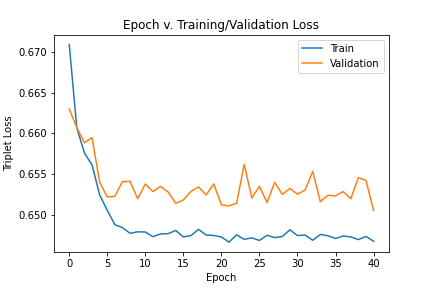
\includegraphics[scale=0.7]{final-report-images/triplet_training.png}
\caption{Dog Comparator Model Training Using a Triplet Loss Function}
\label{fig:x epoch_v_map}
\end{figure}
To assess how well the dog comparator model performed, we first computed the optimum classification threshold by computing the approximate $knee$ of the ROC curve on the validation data to minimize the false positive rate and maximize the true positive rate.  The ROC curve is vizualized below in Figure \ref{fig:x val roc curve}.  We chose a classification threshold of 0.79.

\begin{figure}[h]
\centering
	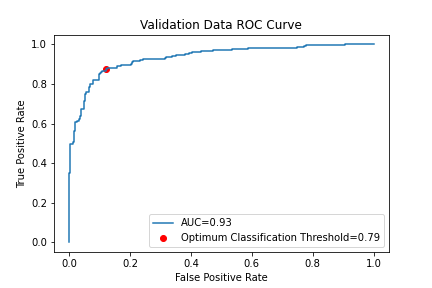
\includegraphics[scale=0.7]{final-report-images/roc_curve_validation_triplet.png}
\caption{Validation ROC Curve Using a Triplet Loss Function}
\label{fig:x val roc curve}
\end{figure}

\noindent It should be noted that the reader may question why the optimum classification threshold is so high.  This is due to the significant dissimilarity between all images even of the same dog in the training data.  By placing no constraints on the type of images in the data-set set, all images had some degree of dissimilarity due to the variety of positions of each dog as well as the backgrounds in each image.  As a result, we found that similar dogs tended to have a similarity value near or slightly above 0.5 while dissimilar dogs had a similarity value near one.  

Returning to the assessment of the model, using a classification threshold of 0.79 resulted in a strong test accuracy and F1 score of approximately 0.87 and 0.87 respectively.  However, after examining the similarity values of the model on the validation data we found it did not do well in grouping the comparisons between the same dogs and the comparisons between different dogs.  This is vizualized below in the line plot contained in Figure \ref{fig:x triplet lineplot} where we can see fairly significantly overlap between both groups.

\begin{figure}[h]
\centering
	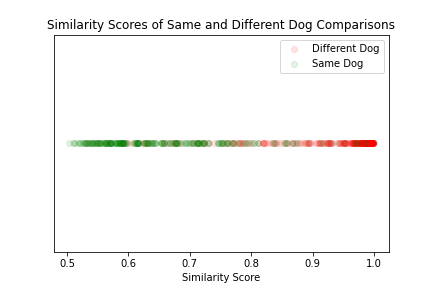
\includegraphics[scale=0.7]{final-report-images/triplet_lineplot.png}
\caption{Line Plot of Similarity Scores Using a Triplet Loss Function}
\label{fig:x triplet lineplot}
\end{figure}
\noindent To remedy this, we retrained our model for 49 epochs with the same parameters as above using a cross entropy loss, and adjusted the individual batch elements to randomly select two images of the same dog, or two images of different dogs with equal probability.  Using the same methodology, we determined the optimum classification threshold to be 0.67.  This resulted in a modest increase in test accuracy and F1 score to 0.89 and 0.89 respectively.  However, this significantly improved the groupings between the comparisons between the same dogs and the comparisons between different dogs. This is shown in Figure \ref{fig:x triplet lineplot}. 

\begin{figure}[h]
\centering
	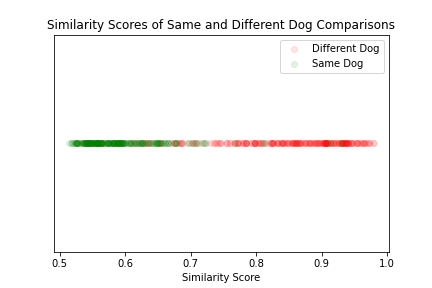
\includegraphics[scale=0.7]{final-report-images/crossentropy_lineplot.png}
\caption{Line Plot of Similarity Scores Using a Cross Entropy Loss Function}
\label{fig:x triplet lineplot}
\end{figure}
\noident We also note that the accuracy of $89\%$ is highly comparable compared to models created by Mougeit, Li and Jia that had an accuracy $91\%$ and $92\%$ \cite{MougeotGuillaume2019ADLA}.  Furthermore, while we concede that our model features a $3\%$ decrease in accuracy, we allow for a far more diverse set of images by not applying our model solely on front facing images of dog faces.

However, an observant read will note that by using images from two randomly selected dogs during both the training and testing processes differing between dogs is an easy task for the model.  This is because dogs of different breeds tend to be very dissimilar and as a result telling them apart is easy.  To account for this, we performed additional testing of our model by testing the performance of the model over different dogs that are known to be similar.  To do this we adjusted the generation of a single batch such that when two images of different dogs are produced, the dogs are of the same breed.  Thus producing two similar dogs.  The model then achieved a significantly decreased but still respectable classification accuracy and F1 score of 0.79 and 0.77 respectively.   To attempt to improve this we trained the model for an additional four epochs on the augmented training data and saw no improvement.  Upon further inspection, we found a crucial flaw in the data.  The data is biased towards the most popular dog breeds where the top three most populous dog breeds account for approximately 50 \% of the dogs in the data-set.  The frequency of the top three least and most populous breed as percentages are vizualized below in Figure \ref{fig:x breed distr}.

\begin{figure}[]
\centering
	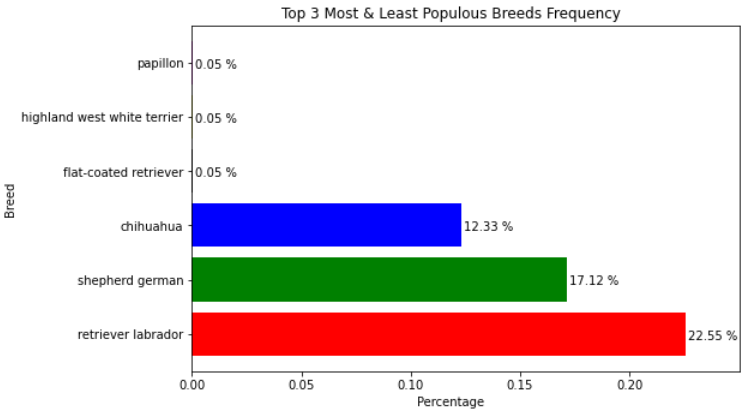
\includegraphics[scale=0.7]{final-report-images/breed_distr.png}
\caption{Top \& Bottom 3 Most Populous Breed Percentage}
\label{fig:x breed distr}
\end{figure}

\newpage

We theorize that by performing additional training by breed we only further biased the model towards these dogs.  Unfortunately, we are not able to account for this flaw in the data.  This is because in other data-sets, one could augment the data by adding random samples from the underrepresented groups with an additional degree of random variation as well.  However, in this case this we are unable to do this without creating two significant issues.  The first, is that by adding random samples of the underrepresented breeds we risk over-fitting the model to specific dogs.  We suspect this would occur because some of the underrepresented breeds have only a few instances and thus adding random samples of these breeds would require randomly sampling the same dogs many times.  The second, is by adding some degree of variation to the images of the randomly sampled dogs the images would likely be distorted significantly.  It should be noted that there is a possible solution to this.  We theorize that unique images of underrepresented breeds could be generated using a generative adversarial network.  However, this is outside the scope of this project.

To investigate the bias of the model towards the most populous dogs, we divided the test data into two groups.  The first contained dogs from the top three most populous breeds and the second contained dogs from all other breeds.  We then applied the model on each group and recorded the results below in Figure \ref{fig:x breed score}


\newpage

\begin{figure}[]

\begin{center}

\begin{tabular}{|l|l|l|}
\hline
                          & \textbf{F1} & \textbf{Accuracy} \\ \hline
\textbf{Top 3 Breeds}     & 0.85        & 0.86              \\ \hline
\textbf{All Other Breeds} & 0.91        & 0.90              \\ \hline
\end{tabular}
\end{center}


\caption{Model Accuracy \& F1 Score by Breed Group}
\label{fig:x breed score}
\end{figure}

\noindent Surprisingly, the model performs better on the second group.  We theorize this is because the second group contains dogs from a multitude of different breeds.   As a result the similarity between every pair of different dogs is greater and thus the model can better differentiate between them.  To test this, we performed the same experiment as before except we added the requirement such that when selecting a pair of different dogs, the dogs must be of the same breed.  The results are shown in Figure \ref{fig:x breed score in breed}.

\begin{figure}[]

\begin{center}

\begin{tabular}{|l|l|l|}
\hline
                          & \textbf{F1} & \textbf{Accuracy} \\ \hline
\textbf{Top 3 Breeds}     & 0.83        & 0.84              \\ \hline
\textbf{All Other Breeds} & 0.74        & 0.78              \\ \hline
\end{tabular}
\end{center}
\caption{Model Accuracy \& F1 Score by Breed Group & Selection within Breeds}
\label{fig:x breed score in breed}
\end{figure}

\noident  There is a clear decrease in model performance between the top three most populous breeds and all others.  Thus, the model does exhibit some bias towards the most populous breeds.  However, the difference is reasonably small at approximately 10 \% with respect to the $F1$ score.



\section{Evaluation}
To evaluate the accuracy of the data product, we have devised an experiment to assess how well the three models work together to match lost and found dogs.  To do this, we first took the entire validation split from the Petfinder data-set and designated every dog as lost.  At the same time, we randomly designated 10 \% of these dogs as found.  For every lost dog we randomly selected an image to use as input and for every found dog we randomly selected a different image to use as input as well.   All three models were then applied over three a grid of parameters to determine the optimum hyper parameter combination to maximize the success rate of matching lost and found dogs.  To be succinct, we varied the number of the most likely breeds recorded for lost and found dogs over a range from one to ten respectively and varied the number of results returned to the user from one to fifteen.  For every combination we determined the success rate of matching lost and found dogs.  A success was defined as the found dog being among the lost dogs returned to the user.  It is assumed if the found dog was among the lost dogs returned to the user, the user would be able to identify the correct dog.  

We found that by recording only the most likely breed for both lost and found dogs, as well as returning the top 15 matches to the users resulted in the highest success rate of 90\% on the validation data.  Unsurprisingly, the success rate improved linearly with the number of matches returned with the user.  Surprisingly however, the highest success rates were achieved by recording the least amount of the top breeds for both lost and found dogs.  This clearly indicates the impact of the Dog Classifier acting as a filter for the Dog Comparator.  This is vizualized below in Figure \ref{fig:x breed comparisons} where the the number of top breeds recorded for both lost and found dogs have been multiplied together into a single number to give the number of comparisons made relative to breeds.  This is shown along the x-axis.  Along the y-axis, the average accuracy for every number of breed comparisons is shown.  We can clearly see that as the number of breed comparisons increase, the accuracy decreases.

\begin{figure}[]
\centering
	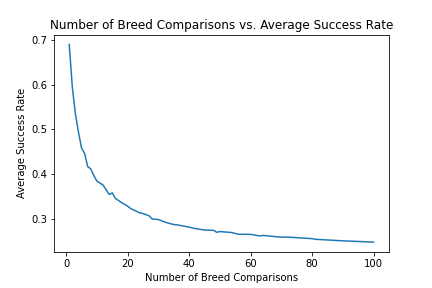
\includegraphics[scale=0.7]{final-report-images/num_breed_comparison_accuracy.png}
\caption{Number of Breed Comparisons vs. Average Success Rate}
\label{fig:x breed comparisons}
\end{figure}

Using the optimum parameter combination as determined over the validation split of recording only the most likely breed for both lost and found dogs and returning the top 15 matches to the user, we achieved a success rate of 89\% on the test split.  We do note the significantly decreased success rate over the test split compared to the validation split is due to the significantly increased size of the test split.  The test split is two times the size of the validation split and as a result the difficulty of finding the found dog among the lost dogs is significantly more difficult.  However, after achieving a final success rate of 89\% we suspect that the true success rate is actually significantly higher in the real world.  This is because of two reasons.  The first is that in this experiment, we are applying this experiment using a single image for both lost and found dogs.  In reality, we expect users would submit multiple images in either case and thus significantly increasing the success rate.  Unfortunately, we are unable to account for this because many dogs in the data-set have only two images.  The second is that in this experiment we are not filtering by location.  By filtering by location before applying the Dog Comparator, the number of false matches would be significantly reduced.  Thus, significantly increasing the success rate.

\newpage

\section{Lessons Learnt}

\section{Summary}

\newpage

\bibliographystyle{unsrt}
\bibliography{references}



\end{document}
